%\appendix
\documentclass[12pt,english]{article} %12 pt for Ecology %
\usepackage[utf8]{inputenc}

\usepackage{geometry}                		
\geometry{verbose,letterpaper,tmargin=2.54cm,bmargin=2.54cm,lmargin=2.54cm,rmargin=2.54cm}   % 1 inch margins for Ecology   

\usepackage{multirow}
\usepackage{graphicx}		
\graphicspath{ {c:} }
\usepackage{setspace}
\usepackage[version=4]{mhchem}
\doublespace
\usepackage{siunitx}
\usepackage[
  backend=biber,
  style=apa,
  maxcitenames=2,
  natbib=true]{biblatex}
\addbibresource{citations.bib}
\usepackage{amsmath}
\usepackage{bm}
\usepackage{amsfonts}
\usepackage{lineno}
\usepackage{gensymb}
\usepackage[sharp]{easylist}%makes nice outlines.  Use # for symbol
\usepackage{blkarray}
\usepackage{lastpage}
\usepackage{times} % times new roman%
\usepackage{lineno} % add line numbers%

\begin{document}


\noindent\textbf{Journal}: Ecology; \textbf{Article Type}: Statistical Innovations

{\Large \noindent \bf %Approaches for handling missing data in ecological time series
Accounting for missing data in autoregressive models of ecological time series
}

%Journal name
%Manuscript type

\medskip

\noindent Alice E. Stears\textsuperscript{*, 1, 2}, 
Melissa DeSiervo\textsuperscript{*, 3, 2},
Dustin Gannon\textsuperscript{4, 2},
Amy Patterson\textsuperscript{5, 2},
Alice M. Carter\textsuperscript{6,7},
Joanna R. Blaszczak\textsuperscript{8},
Matt Trentman\textsuperscript{9},
Eliza Grames\textsuperscript{10},
Robert O. Hall, Jr\textsuperscript{7},
Joshua P. Jahner\textsuperscript{11, 2},
Saheed O. Jimoh\textsuperscript{2},
Courtenay A. Ray\textsuperscript{2},
Christa L. Torrens\textsuperscript{7},
Lauren Shoemaker$^{\circ}$\textsuperscript{2},
Christopher Weiss-Lehman$^{\circ}$\textsuperscript{2}

\noindent\noindent \textbf{Author affiliations}

\noindent\textsuperscript{1} Center for Adaptable Western Landscapes, Northern Arizona University, Flagstaff, AZ

\noindent\textsuperscript{2} Botany Department, University of Wyoming, Laramie, WY

\noindent\textsuperscript{3} Biology Department, Union College, Schenectady, NY

\noindent\textsuperscript{4} Department of Forest Ecosystems and Society, Oregon State University, Corvallis, OR 

\noindent\textsuperscript{5} Department of Biology, University of Maryland, College Park, MD

\noindent\textsuperscript{6} Department of Mathematics and Statistics, Utah State University, Logan, UT

\noindent\textsuperscript{7} Flathead Lake Biological Station, University of Montana, Polson, MT

\noindent\textsuperscript{8} Department of Natural Resources and Environmental Sciences, University of Nevada, Reno, Reno, NV

\noindent\textsuperscript{9} O’Connor Center for the Rocky Mountain West, University of Montana, Missoula, MT

\noindent\textsuperscript{10} Biological Sciences, Binghamton University, State University of New York, Binghamton, NY

\noindent\textsuperscript{11} Department of Biology, New Mexico Institute of Mining and Technology, Socorro, NM

\noindent\textsuperscript{*} Denotes equal contribution as lead author

\noindent{$^{\circ}$} Denotes equal contribution as primary investigator

\noindent \textbf{Corresponding author}: Alice Stears, alice.e.stears@gmail.com 


\section*{Appendix S1}


\subsection*{Introducing Missingness}

We created MCAR datasets with varying proportions of missing data and degrees of autocorrelation in missingness (Fig. \ref{fig:missingtypes} B--E) by viewing a time series as a Markov-modulated Bernoulli process where the variable could have two states: missing or not missing \citep{Gharib2014, Edwards1960}. The probability that an observation in a time series at time $t+1$ was missing depended on both the specified proportion of non-missing values in the entire time series ($p$) and the specified degree of autocorrelation in missingness ($\omega$). In a time series $X_1, X_2, ..., X_n$, the transition matrix that describes the probability of an observation at $X_{t+1}$ being missing, based on whether the observation at $X_t$ was missing is defined as: 


\begin{equation}
\begin{blockarray}{rcccc}
\text{} & \BAmulticolumn{4}{c}{X_{t+1}}\\
X_t & \text{Present} & \text{Missing}  \\
\begin{block}{r(cccc)}
\text{Present} & 1-(1-\omega)p & (1-\omega)p \\
\text{Missing} & (1-\omega)(1-p) & \omega + (1-\omega)p  \\
[1ex]
\end{block}
\end{blockarray}
\end{equation}


We created MNAR datasets with various proportions of msising data by first calculating the mean and standard deviation of the time series with no missing data, then using these point estimates as the mean and standard deviation of a normal distribution. We then identified the quantiles of that normal distribution above and below which the density of the normal distribution corresponded to the desired proportion of missingness. We replaced any values above and below those quantiles with an NA.

\subsection*{Missing Data Approaches} 
\textbf{Simple and Complete Data Deletion}: The ``simple data deletion" approach involves removing missing values from a time series, compressing the dataset, and running the model as if the time intervals between observations were all equal (Fig. 1 A). This method violates the assumption of equal temporal spacing between observations, an assumption implicit in most time series models. We include it here as a reference because it is simple and commonly used in published studies. We also include ``complete case data deletion," which maintains equal spacing between observations by removing a missing value itself as well as the subsequent observation(s) that is predicted by the missing value (Fig. 1 A). However, those observations after a missing value are retained as predictors of the subsequent observation(s). 

\textbf{Multiple Imputation}: Multiple imputation (MI) is an approach that systematically fills in missing observations with imputed values, and creates several versions of complete data sets that can be used to estimate uncertainty around each imputed value (Fig. 1 B). MI is commonly used in ecology, with multiple studies evaluating methods and approaches to conduct MI for functional traits \citep{taugourdeau_filling_2014,johnson_handling_2021,penone_imputation_2014}, population biology \citep{onkelinx_working_2017}, time series \citep{hui_gap-filling_2004}, and meta-analyses \citep{ellington_using_2015}. Multiple Imputation’s (MI) effectiveness can depend on the number of imputed datasets (\textit{m}). It is often assumed that \textit{m}=5 is a minimum value \citep{honaker_what_2010}; however, researchers have used \textit{m}=200 when comparing methods in the ecological sciences \citep{onkelinx_working_2017}. In general, larger values of \textit{m} result in more accurate estimates of both parameter values and uncertainty. However, increasing \textit{m} results in a trade-off between accuracy and computation time; this can be particularly problematic for data-rich (e.g., long time series) or complex (e.g., hierarchical) models. 
After imputing the \textit{m} data sets, the analyses of interest are confronted with each data set, and the estimated parameters from the \textit{m} analyses are averaged using Rubin rules of averaging to get the parameter(s), and associated uncertainty, from which inference can be made. We implemented multiple imputation with the Amelia II package in R \citep{honaker2011}, which uses an expectation maximization algorithm (see below) in combination with a bootstrapping technique for deciding what values to impute. We used $m=5$ in order to provide decent estimates without excessive run times.

For both the simulated and empirical population count time series, since we did not have any covariates, the only variables used for imputation were the population size at time \textit{t} and population size at time \textit{t-1}. For time series with chunks of missing data, the Amelia multiple imputation function had to be run iteratively, with missing values filled in from the edges of the missing chunks. In addition, while the recommended settings for dealing with time series data using the Amelia package include incorporating preceding and proceeding time points by specifying the ``lags" and ``leads" options \citep{honaker2011}, it was not possible to use the lags option, since the current population was already using the population at the previous point as its only predictor for imputation. Instead, we included only the leads option, which still resulted in occasional failure of the method at extremely high levels ($>70\%$) of missing data due to excessive collinearity between the preceding and proceeding time points. The lack of error handling for extremely collinear variables is an unfortunate issue for this method when using data sets without covariates, or data sets with highly collinear covariates.  

For both the simulated and empirical Gaussian series, implementing multiple imputation was more straightforward since an observation at time \textit{t} was informed by two covariates in addition to the observation at the time \textit{t-1}. In this case, we were able to use both the ``lags" and ``leads" options in \texttt{amelia}. 

Following execution of MI using Amelia II, we fit statistical models to time series following the methods described in \textbf{Main Text: Comparing missing data approaches}.

\textbf{Kalman Filter}: The Kalman Filter (KF) was developed to estimate the state of a dynamic system that is observed with error but can be used to derive the likelihood function of a time series with missing observations (Fig. 1 C). To illustrate the approach, assume a state-space model

\begin{equation}
    \begin{aligned}
        X_t &= \phi X_{t-1} + \epsilon_t \\Y_t &= X_t + e_t
    \end{aligned}
\end{equation}
where $X_t$ is the true ``state" of the system at time $t$, $Y_t$ is the observed value at time $t$, and $\epsilon_t \sim \mathcal{N}(0, \sigma^2)$ and $e_t \sim \mathcal{N}(0, \tau^2)$ are IID white noise error terms for the process and observation error, respectively. The Kalman Filter is primarily focused on estimating the unobserved state of the system, $X_t$, and can be conceptualized as a two-step procedure in which, given an initial state $X_0$, we can forecast the next state $X_1$. Then, following data collection at the next time point, $y_1$, we update the forecast using Bayes' theorem. Specifically, the forecast distribution for $X_1$ is
\begin{equation}
    p(x_1) = \int p(x_1 | x_0)p(x_0)dx_0
\end{equation}
where $p(\cdot)$ denotes the probability density function. Assuming IID Gaussian errors, $p(x_1)$ is normal with mean ${\tilde x}_1 = \phi x_0$ and variance $v_1 = \phi^2 \frac{\sigma^2}{1 - \phi^2} + \sigma^2$. Given the observed value $y_1$, we update the estimate of $X_1$ using Bayes theorem
\begin{equation}
    \begin{aligned}
        p(x_1 | y_1) &\propto p(y_1 | x_1) p(x_1)
        &= \mathcal{N}\Bigl(\tilde x_1 + K_1(y_1 - \tilde x_1),\ (1 - K_1)v_1 \Bigr)
    \end{aligned} 
\end{equation}
where $K_1 = v_1 / (v_1 + \tau^2)$ is the \textit{Kalman gain} and creates a weighted average of the forecast and observation. %If the observation error is large, the forecast is favored as an estimate of $X_t$, whereas if the process noise is large relative to the observation error, the estimate of $X_t$ tends towards the observed value $y_t$.
For our focus on missing data, we assume the process is observed without error such that $Y_t = X_t$ and $\tau^2 = 0$. Without observation error, the Kalman gain $K_t = 1$ for all $t$ since $\tau^2 = 0$, and $p(x_1 | y_1) = \mathcal{N}(y_t, 0)$. Thus, the update step gives complete information about $X_t$, and the likelihood function can be defined based on the data $y_1,...,y_n$. However, if data are missing, the update step cannot occur. So, in the case of missing data without observation error, the Kalman Filter alternates between pure forecast steps when data are missing and pure ``update" steps when data and the state of the system are completely observed, but the forecast steps yield a method for computing the likelihood function recursively without needing to know the states of $X_t$ in which we were unable to observe the process and therefore have no associated $y_t$.

The Kalman filter assumes a Gaussian error distribution, so we only used this method with the simulated and empirical real-valued time series. We implemented KF missing data approach at the same time as the model fitting process, where we fit an AR(1) model with two covariates using the \texttt{arima} function from the \texttt{stats} package in R \citep{r_2021} (KF is the default algorithm used to handle missing values in this R function). 


\textbf{Expectation Maximization}: The expectation maximization (EM) algorithm is an iterative algorithm that is conceptually similar to KF, and recursively computes the likelihood of a time series with missing data (Fig. 1 D). Given an initial guess for the parameter vector we wish to estimate, ${\bm \theta}_0$, the first step (Expectation step) proceeds to ``fill in" the missing observations with their expectation given the observed data and the initial parameter vector ${\bm \theta}_0$ %. For example, if $Y_t$ were missing, we impute $Y_t$ with $\mathbb{E}(Y_t | y_{t-1}, {\bm \theta}_0)$
, which is equivalent to the forecast step of the Kalman filter conditioned on ${\bm \theta}_0$. In the second step (maximization step), we compute the maximum likelihood estimate of ${\bm \theta}$ using the filled-in time series as data to give an updated estimate $\hat {\bm \theta}_1$. We then iterate this process, updating the forecasts of the missing data using their expectations conditional on $\hat {\bm \theta}_1$, then maximizing the likelihood with respect to $\bm \theta$ using the time series filled-in with the updated forecasts. This process is iterated until the difference between successive estimates is acceptably small, indicating convergence (that is, $||\hat {\bm \theta}_i - \hat {\bm \theta}_{i-1}||_1 < \delta$ for some small $\delta > 0$).

Given its similarity to KF, we only used this missing data approach for the simulated and empirical times series of counts. We constructed an approximate EM algorithm to estimate the parameters of the Ricker model in which missing data were rounded to the nearest integer value during the expectation step such that the likelihood was well-defined for the filled-in series. As such, the missing data were dealt with at the same time as the model fitting process. We used the \texttt{optim} function from the \texttt{stats} package in \texttt{R} for the maximization step \citep{r_2021}. %In Figure S2%\ref{fig:EM-bias-checks}
%, we show that the estimates are asymptotically unbiased. 
Note that the algorithms required to estimate standard error of parameter estimates generated from EM are notoriously unstable and difficult to implement in R, so the results of models we fit using this missing data approach do not include standard error estimates. 

\textbf{Data Augmentation}: Data augmentation (DA) provides a model-based framework for estimating missing observations as well as the parameters of interest, but comes with the added benefit of standard errors for the estimates of all the unknown quantities by treating the missing observations as additional parameters to be estimated (Fig. 1 D). We fit the Gaussian AR(1) models with DA and Stan \citep{carpenter_stan_2017} by using the rstan \citep{rstan_package} and brms \citep{burkner2017brms} packages in R \citep{r_2021}. Data augmentation for the population model is not possible with Stan, however, due to the requirement of continuous parameter space for the Hamiltonian Monte Carlo (HMC) methods Stan uses to sample the posterior distribution (at least not without marginalizing out the discrete parameters, which proved intractable). Treating missing integer data as parameters was therefore not possible with Stan, and partially-known parameter vectors are not supported in JAGS. We therefore designed a Gibbs sampler with Metropolis updates for the log growth factor ($r$) and intra-specific competition coefficient ($\alpha$), and Gibbs sampling of any missing observations, $N_{t}^{(0)}$, conditional on $(r, \alpha, {\bf N}_{t-})$, where ${\bf N}_{t-}$ is the vector of abundances (both observed and unobserved) up to but not including time $t$. We used weakly informative Gaussian priors for $r$ and $\ln(\alpha)$ and fit the models using custom functions written in R. 


\printbibliography

%\bibliographystyle{ecology}
%\bibliography{citations}


\renewcommand{\figurename}{Figure}
\renewcommand{\thefigure}{S\arabic{figure}}
\begin{figure}
     \noindent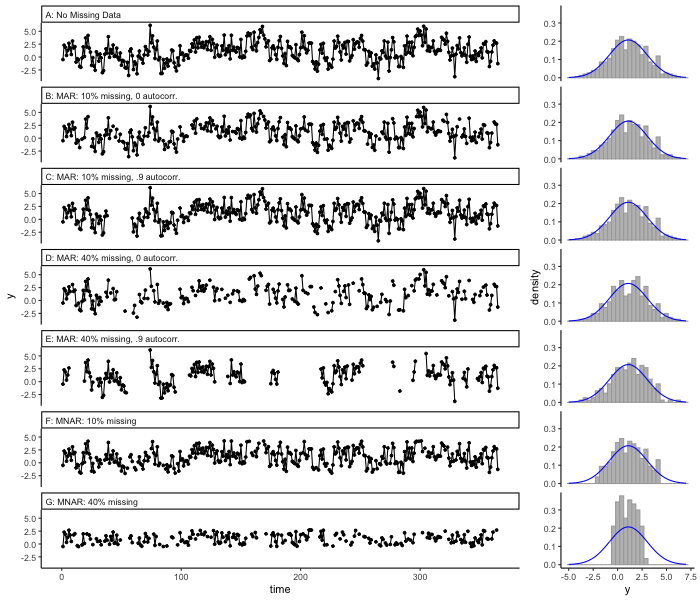
\includegraphics[width = 0.85\textwidth]{Figures/CompareMissingnessTypes_fig.png}
     \caption{An example time series demonstrating different types and amounts of missing data. The left column shows the same time series with different amounts and types of missingness and right column shows the distribution of data points in each resultant time series. A. Complete time series with no missing data. Rows B through E show the time series with 10\% (B and C) or 40\% (D and E) of data missing completely at random (MCAR), with either low autocorrelation in missing data (B and D) or high autocorrelation (C and E). Rows F and G show the time series with data missing not at random (MNAR) for 10\% missing data (F) and 40\% missing data (G).}
     \label{fig:missingtypes}
 \end{figure}

 \begin{figure}
     \noindent\includegraphics[width = 0.85\textwidth]{Figures/MockedUpFigures/heatmap_GaussianMCAR_all.png}
     \caption{Median error of parameter recovery, median absolute error, and model coverage of $\phi$ and $\beta$, depending on the proportion of missing data and autocorrelation in missingness for each of five missing data approaches, using simulated, real-valued datasets with data missing completely at random (MCAR).}
     \label{fig:GaussianMCARheatmapALL}
 \end{figure}

  \begin{figure}
         \noindent\includegraphics[width = 0.85\textwidth]{Figures/MockedUpFigures/heatmap_PoissonMCAR_all.png}
     \caption{Median error of parameter recovery, median absolute error, and model coverage of $\alpha$ and $r$, depending on the proportion of missing data and autocorrelation in missingness for each of five missing data approaches, using simulated time series of counts with data missing completely at random (MCAR). Note that coverage is not shown for the Expectation Maximization approach, since most implementations of this method do not include estimates of standard error.}
     \label{fig:PoissonMCARheatmapALL}
 \end{figure}
 
%\subsection{Bias due to endogeneity}

%It is well known that the ordinary least squares estimator (OLS) of the autoregressive coefficients in an AR($p$) model is biased. To see this, consider a simple AR(1) model with mean zero and variance of the innovations $\sigma^2$. The model can be written as
%$$
%y_t = \phi y_{t-1} + \epsilon_t
%$$
%where $\epsilon_0, ..., \epsilon_n \overset{iid}{\sim} \mathcal{N}(0, \sigma^2)$ and $\phi$ is the autoregressive coefficient. The OLS estimator of $\phi$, $\hat{\phi}$ is obtained by regressing observations $y_1,...,y_n$ against $y_0,...,y_{n-1}$. Thus, the OLS estimator can be written as
%\begin{equation*}
%    \begin{aligned}
%        \hat{\phi} &= \frac{\sum_{t=1}^n y_t y_{t-1}}{\sum_{t=1}^n y_{t-1}^2}\\
%        &= \frac{\sum_{t=1}^n (\phi y_{t-1} + \epsilon_t) y_{t-1}}{\sum_{t=1}^n y_{t-1}^2}\\
%        &= \frac{\sum_{t=1}^n (\phi y_{t-1}^2 + \epsilon_t y_{t-1})}{\sum_{t=1}^n y_{t-1}^2} \\
%        &= \phi \frac{\sum_{t=1}^n y_{t-1}^2}{\sum_{t=1}^n y_{t-1}^2} + \sum_{t=1}^n \frac{y_{t-1}}{\sum_{t=1}^n y_{t-1}^2} \epsilon_t\\
%        &= \phi + \sum_{t=1}^n \frac{y_{t-1}}{\sum_{t=1}^n y_{t-1}^2} \epsilon_t.
%    \end{aligned}
%\end{equation*}
%Taking the expectation,
%\begin{equation*}
%    \mathbb{E}(\hat \phi) = \phi + \mathbb{E}\left(\sum_{t=1}^n \frac{y_{t-1}}{\sum_{t=1}^n y_{t-1}^2} \epsilon_t \right)
%\end{equation*}
%we see that, because the sum in the denominator of the second term in the expectation, $\sum_{t=1}^n y_{t-1}^2$, is not independent of $\epsilon_t$ (if $\epsilon_t$ is large and positive, the sum in the denominator will also increase), the ``covariate" we use is \textit{endogenous}, meaning it is not independent of the errors. The negative correlation between $\epsilon_t$ and the reciprocal of sum $\sum_{t=1}^n y_{t-1}^2$ results in a downward-biased estimator of $\phi$ (i.e, closer to zero). 




\newpage


\end{document}